\nonstopmode
\documentclass{minimal}
\def\pgfsysdriver{pgfsys-tex4ht.def}
\usepackage{tikz}
\usetikzlibrary{arrows}
\begin{document}
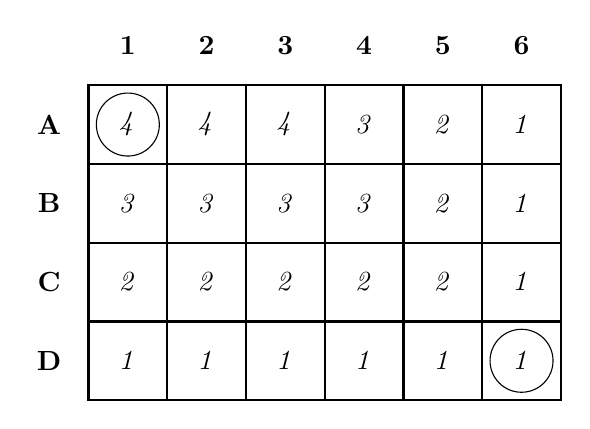
\begin{tikzpicture}

\begin{scope}[thick]
\foreach \x in {1,...,6}
  \foreach \y in {1,...,4}
  {
    \draw (\x,\y) +(-.5,-.5) rectangle ++(.5,.5);
  }
\end{scope}

\foreach \x in {1,...,6} \draw (\x,5) node{\textbf{\x}};
\draw (0,4) node{\textbf{A}};
\draw (0,3) node{\textbf{B}};
\draw (0,2) node{\textbf{C}};
\draw (0,1) node{\textbf{D}};

\foreach \x in {1,...,6} \draw (\x,1) node{\textit{1}};
\foreach \y in {2,...,4} \draw (6,\y) node{\textit{1}};
\foreach \x in {1,...,5} \draw (\x,2) node{\textit{2}};
\foreach \y in {3,...,4} \draw (5,\y) node{\textit{2}};
\foreach \x in {1,...,4} \draw (\x,3) node{\textit{3}};
\draw (4,4) node{\textit{3}};
\foreach \x in {1,...,3} \draw (\x,4) node{\textit{4}};

\draw (1,4) circle (0.4);
\draw (6,1) circle (0.4);

\end{tikzpicture}
\end{document}
